\chapter{Instrumentation}
\label{chap:payload}

The payload subsystem is a crucial part of the VISTA mission. Different scientific goals may be obtained through the use of different equipment. This chapter presents the instruments that will be implemented in the aerial platform. First, a design option tree of the payload instruments is presented in \autoref{sec:DOT_payload}. 

% As part of the payload subsystem, the following requirements must be met during the design process. Such requirements will be addressed in the following sections. The compliance of the different objectives of the VEXAG roadmap goals \cite{VEXAG2019} will also be explored individually.

% \begin{table}[H]
% \centering
% \begin{tabular}{|l|p{9cm}|l|}
% \hline
% \textbf{Requirement ID} & \textbf{Requirement} & \textbf{Parent Requirement} \\ \hline

% REQ-F-SCI-01 & The system shall perform aerosol sampling and detailed chemical analysis of clouds at least once per month. & REQ-STK-1.2 \\ \hline

% REQ-F-SCI-02 & The sampling system shall not affect the chemical composition of the sample. & REQ-STK-1.2 \\ \hline

% REQ-C-SCI-03 & The maximum altitude separation between samples shall be TBD km. & REQ-STK-1.2 \\ \hline

% REQ-C-SCI-04 & The altitude accuracy of sampling shall be TBD km. & REQ-STK-1.2 \\ \hline

% REQ-C-SCI-05 & The S/C shall be able to measure vertical wind speed at TBD intervals & REQ-STK-1.2 \\ \hline

% REQ-F-SCI-06 & The S/C shall include TBD measurement systems to detect any seismic activity & REQ-STK-1.2 \\ \hline

% REQ-F-SCI-07 & The S/C shall be able to measure cloud dynamics at TBD intervals & REQ-STK-1.2 \\ \hline

% REQ-F-SCI-08 & The S/C shall be able to measure horizontal wind speed at TBD intervals & REQ-STK-1.2 \\ \hline

% REQ-F-SCI-09 & The mission shall address the VEXAG roadmap goals & REQ-STK-1.2 \\ \hline

% REQ-F-SCI-10 & The S/C shall be able to measure the temperature of the venusian atmosphere & REQ-STK-1.2 \\ \hline

% REQ-F-SCI-11 & The S/C shall be able to measure pressure of the venusian atmosphere & REQ-STK-1.2 \\ \hline

% REQ-C-PAY-01 & Each instrument suite shall achieve a successful analysis probability greater than 80\%. & REQ-STK-1.5 \\ \hline

% REQ-C-PAY-02 & The total mass of the payload shall stay below TBD kg. & REQ-STK-1.1 \\ \hline

% REQ-F-PAY-03 & Scientific components shall fit within the TBD volume of the allocated space. & REQ-STK-1.1 \\ \hline

% REQ-F-PAY-04 & The generated payload data that needs to be stored shall be no more than TBD MB. & REQ-STK-1.3 \\ \hline

% \end{tabular}
% \caption{Science and Payload Requirements}
% \label{tab:science_payload_requirements}
% \end{table}

\section{Design Option Tree of Payload Instruments}
\label{sec:DOT_payload}

The main scientific goals of VISTA involve two main areas of research. The first proposes the deep understanding of the chemical composition of the atmosphere, which involves the study of Venusian cloud dynamics, pressure, temperature, and wind speed. Moreover, conducting aerosol sampling and detailed chemical analysis of the upper and/or middle cloud layer periodically is required. The second area of study involves the continuous investigation of the seismic and/or tectonic activity on the planet. Apart from the aforementioned scientific goals, VISTA also aims to address with the VEXAG roadmap goals. All these factors will be taken into account when selecting the possible options. 

Based on these two bigger branches of investigation, different measurement techniques can be proposed to achieving such goals. The scientific instrumentation options for the payload design are presented in the design option tree illustrated in \autoref{fig:dot_payload}. The tree is divided into the two main instrumentation subdivisions. The methods presented in the tree pertain to all possible methods for investigation from a balloon aerial platform. In the following subsections, the rationale of why each method has been deemed feasible, unfeasible or why it is the selected method is discussed. Such explanation takes into account the Venusian conditions to which the instruments will be subjected as well as their overall scientific output. The final design choices are also justified under the same section.

% 
\includepdf[pages=-]{"fig/WFD-DOT_payload.drawio22.pdf"}

% \begin{figure}[H]
%     \centering

%     \begin{minipage}{0.7\textwidth}
%         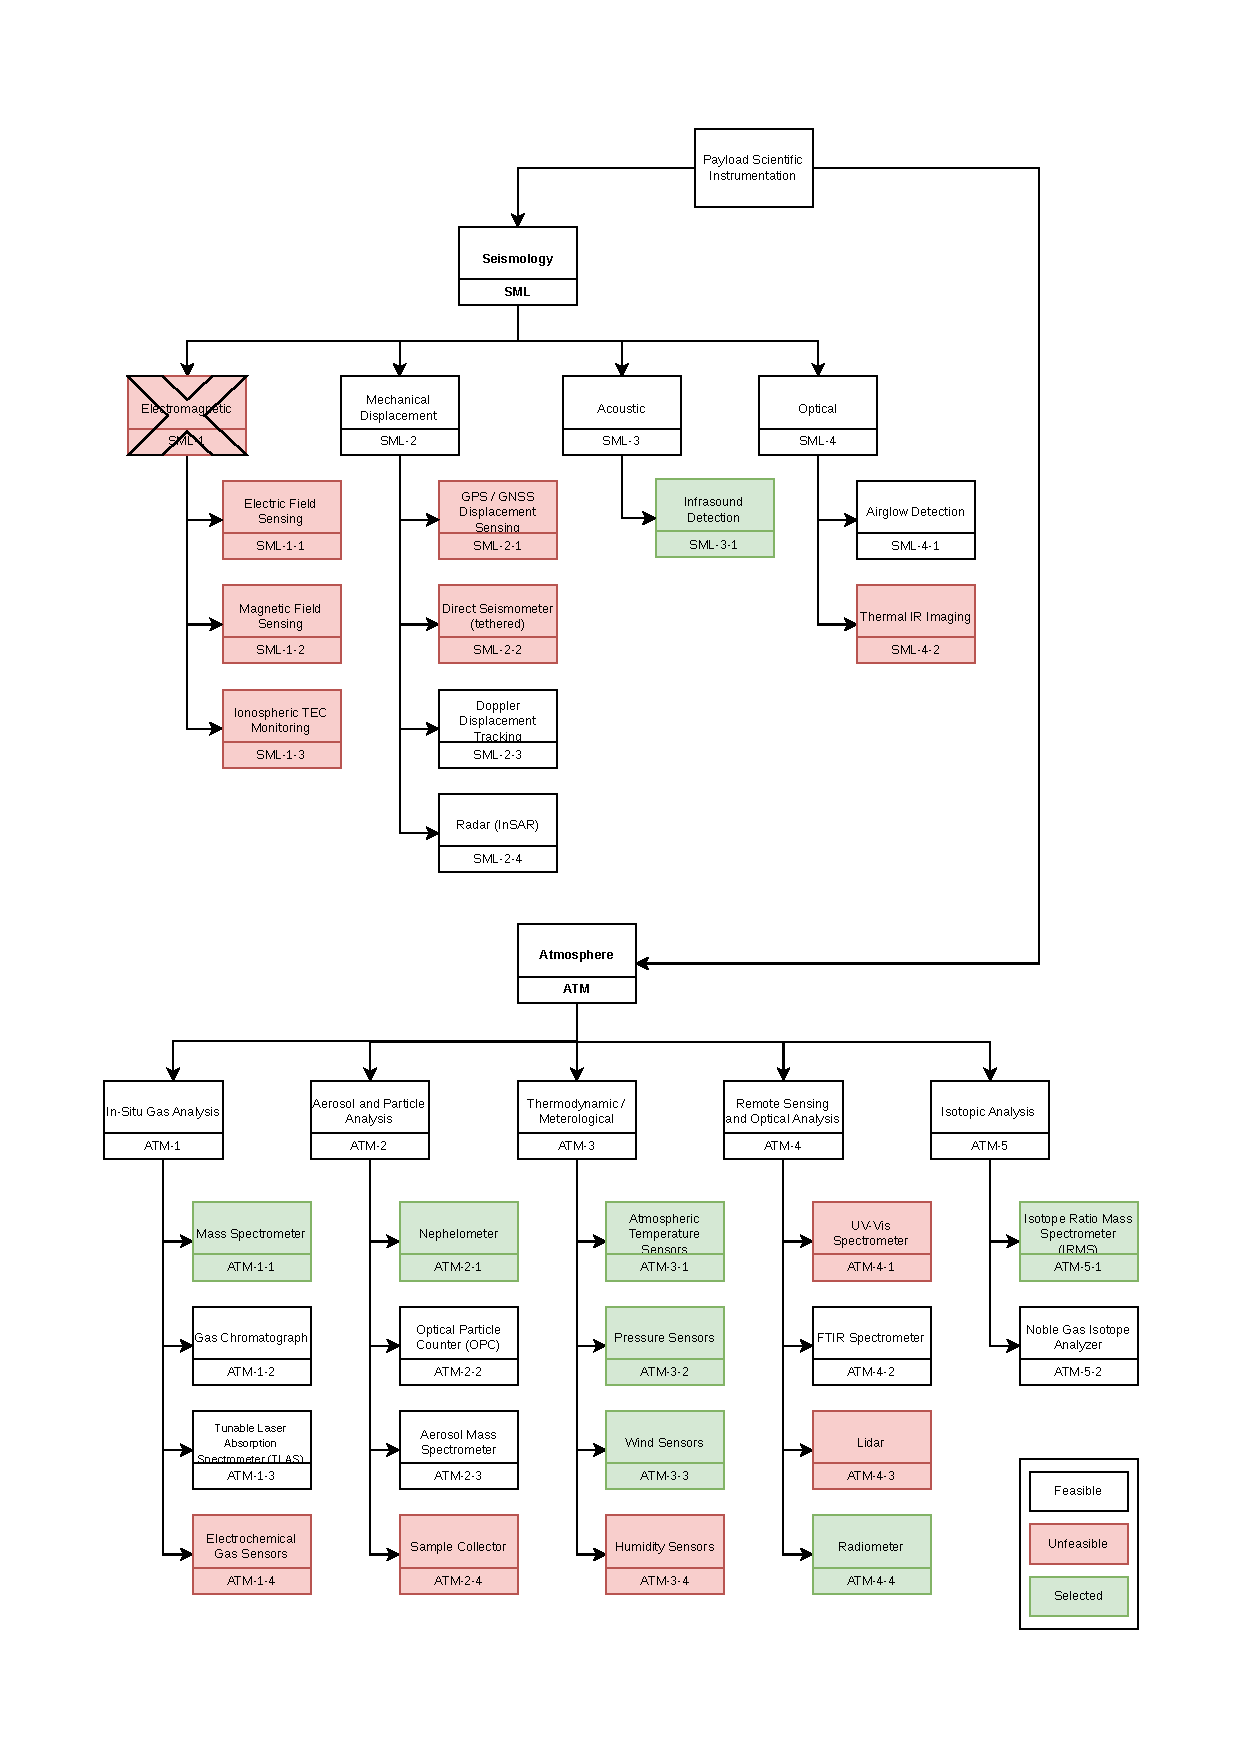
\includegraphics[
%             page=1,
%             width=\linewidth
%         ]{fig/WFD-DOT_payload.drawio22.pdf}
%     \end{minipage}
%     \vfill
%     \begin{minipage}{\textwidth}
%         \caption{Design Option Tree Payload Subsystem}
%         \label{fig:dot_payload}
%     \end{minipage}

% \end{figure}

\subsection{Seismic Measurement}

There are many ways to measure seismic activity from an aerial platform. In \autoref{fig:dot_payload}, a design option tree presents the options for seismology measurements from a balloon. The tree clarifies which options are feasible, unfeasible and the preferred selected options to be further considered on later design stages. The primary modes of measurement include electromagnetic analysis, mechanical displacement detection, acoustic analysis, and optical imaging. Each level has different measuring techniques that are presented as sub-levels in the tree. The rationale and explanation of each method is presented below. 

% The scientific objectives of this part of the VISTA mission and its connection to relevant requirements is presented in \autoref{tab:seismic_objectives}. 

% \begin{table}[H]
% \centering
% \small
% \caption{Seismic science objectives and their links to mission requirements and VEXAG Goals, Objectives, and Investigations.}
% \label{tab:seismic_objectives}

% \renewcommand{\arraystretch}{1.15}
% \setlength{\tabcolsep}{6pt}

% \begin{tabularx}{\textwidth}{|
% >{\raggedright\arraybackslash}X|
% >{\raggedright\arraybackslash}p{5.2cm}|}
% \hline
% \textbf{Science Objective} & \textbf{Relevance} \\
% \hline

% Detection and characterisation of Venusquakes and volcanic eruptions to determine whether Venus is presently seismically and volcanically active, and to constrain the frequency and magnitude distribution of seismic events. &
% VEXAG III.A.2 Geologic Activity; VEXAG I.A.1 Crustal Recycling; REQ-F-SCI-06 \\
% \hline

% Identification of dominant atmospheric gravity-wave source regions and assessment of whether these are topographically controlled, providing insight into surface--atmosphere mechanical coupling on Venus. &
% VEXAG II.A.2 Mesoscale Processes; VEXAG II.A.1 Deep Dynamics; VEXAG III.A.2 Geologic Activity; REQ-F-SCI-06 \\
% \hline

% \end{tabularx}
% \end{table}

For the first level, an option considered is using electromagnetic waves for the detection of seismic activity. A few options that make use of such method were explored, however they were all deemed unfeasible under Venus' conditions, therefore such method will be eliminated from the considered concepts. 

\begin{itemize}
    \item \textbf{SML-1-1}: This method requires measuring dc and very low frequency electric fields. Venus conditions can pose quite a challenge to this method. The high conductivity of the atmosphere due to the high temperatures makes the signals dissipate quickly and electrical circuits tend to short-circuit \cite{SML-1-1}. Moreover, the dense atmosphere and the thick cloud layer may also contribute to signal attenuation and noise production. These factors gravely impacts the ability of accurate measurements and seismic activity detection, therefore such method is considered unfeasible. 
    \item \textbf{SML-1-2}: Venus lacks an intrinsic magnetic field. There may be a very weak induced magnetic field created by the interaction between solar wind and Venus' ionosphere. However, such field is not strong enough for a clear distinguish between noise and electromagnetic waves to be made, therefore such method is also considered unfeasible. 
    \item \textbf{SML-1-3}: Such technique involves the measurement of the total electron content in the ionosphere, however it requires technology not yet present on Venus. This includes a GNSS (Global Navigational Satellite System), as well as extensive ground station coverage \cite{SML-1-3}. For the aforementioned reasons, this methods was also deemed unfeasible.      
\end{itemize}

Another option considered for determining seismic activity involves the measurement of surface displacement due to such geological events. Some techniques are also deemed unfeasible due to the lack of technology present in Venus. Other methods, although still feasible, may present some challenges given the mission conditions. Therefore, using mechanical displacement as primary measurement was discarded. 
\begin{itemize}
    \item \textbf{SML-2-1}: As mentioned previously, Venus does not possess a GNSS or global GPS system, therefore this technique is discarded from the option possibilities. 
    \item \textbf{SML-2-2}: A direct seismometer requires the instrument to be placed near or/and at the surface for accurate measurements to be made. Due to the high temperatures near the surface, no equipment would survive the required mission length. Moreover, a tether of over 50 km is also considered unfeasible for this mission due to its complex engineering implications. 
    \item \textbf{SML-2-3}: 
    \item \textbf{SML-2-4}: This system serves specifically well for ground and topography mapping, as the radio waves are capable of penetrating the cloud layer of Venus. However, such technology may present some limitations for an aerial balloon platform on Venus. In order to detect changes in altitude, repeat orbits are necessary in order to take measurements of the same location. As the balloon presents little to no control capability, and instead flows according to the planet's wind, ensuring repeat orbits is a challenge. 
\end{itemize}

A third category of measurement technique involves the study of the seismo-acoustic waves produced by seismic activity and that are later propagated through the atmosphere. This method shows to be the most promising for future Venus missions. 

\begin{itemize}
    \item \textbf{SML-3-1}: Due to Venus’s dense atmosphere, there is strong coupling between the solid surface and the atmosphere. As these waves travel upward, they preserve key characteristics of the original seismic surface waves, including their frequency content and dispersion. This makes it possible for a balloon platform to obtain accurate and reliable measurements by measuring pressure fluctuations in the atmosphere \cite{SML-3-2}. Therefore, this is a very strong contender for the detection of seismic activity within the possible options. 
\end{itemize}

The fourth, and last, measuring technique considered involves optical analysis of either the upper atmosphere layer of Venus, or the thermal imaging of the surface. 

\begin{itemize}
    \item \textbf{SML-4-1}: This technique presents limitations for an aerial balloon platform, as it requires higher observational altitudes and a larger imaging area of the planet. This approach is more effective when combined with an orbiter, which can provide a much wider field of view due to its higher altitude, enabling continuous monitoring over a defined region. A cooperative system could therefore be preferred, where the orbiter acts as a communication relay and provides global context, while the balloon functions as a local tracking station, offering higher-resolution measurements of atmospheric perturbations \cite{seism1}. Although limited, it still presents as an option for seismic detection.
    \item \textbf{SML-4-2}: As the temperature at the surface is extremely high, over \SI{450}{\celsius}, distinguishing small thermal anomalies provoked by seismic activity on the surface can become very challenging. Due to the high sensitivity to noise of this method, it was determined unfeasible for the mission.
\end{itemize}

Acoustic measurement via infrasound detection is the only feasible seismic sensing method for the VISTA balloon platform. Barometers measure atmospheric pressure fluctuations, which can be directly related to ground motion in the infrasound frequency range. A balloon drifting with the wind experiences reduced background wind noise compared to a fixed station, and atmospheric attenuation in Venus's ($CO_2$) atmosphere is negligible for wave periods above one second. Over the five-year mission duration, even a low seismic event rate of one event per year yields a high detection probability. Infrasound detection is therefore baselined as the primary seismic sensing mode, implemented through the barometer array described in the following sections. Optical instruments coupled with an orbiter remain a complementary option to be explored in later design stages, independent of the current payload subsystem.

% Source Twan:  https://www.sciencedirect.com/science/article/pii/S1270963821001176

% Based on the rationale for each instrumentation method, it can be concluded that only acoustic measurements and optical instruments coupled with an orbiter are feasible to produce the results required for the mission. Even for the remaining feasible options, the challenges that each component impose, makes them not suitable, and therefore, discarded options. 

% Infrasound wave detection presents many advantages when used in the Venus atmosphere compared to other methods. Infrasound detection is achieved by measuring pressure fluctuations in the atmosphere using barometers. In the infrasound frequency range, these pressure variations can be directly related to the underlying ground motion through a proportional relationship. The minimum number of seismic events per year required for wave detection decreases with increasing mission duration. In other words, the longer the mission duration, the greater the likelihood of detecting events, even if they occur infrequently. With the current mission concept lasting five years, and assuming an average of only one geological event per year, the balloon platform would likely already be capable of detecting such seismic signals.

% Regarding wave interference, a balloon drifting with the wind experiences lower background wind noise than a fixed ground station, since the relative wind velocity is reduced. Atmospheric attenuation can also dampen wave energy. In Venus’s atmosphere, this effect is mainly controlled by the relaxation of \(CO_2\) molecules, but it is only significant for acoustic waves with periods shorter than one second \cite{SML-3-2}. This effect will be discussed further in later stages of the design.

% As infrasound wave detection is the most promising approach for an aerial balloon platform within the presented options, this will be used as primary mode for the detection of seismic activity in the VISTA mission. That is, no trade-off will be made for the seismology instruments. Such detection is made through the use of barometers, that can be assembled in many ways. The option for the use of optical instruments may still be explored in later stages, depending on remaining mass and cost budget. However, as this instrument influences mainly the orbiter, such possibility can be considered independent of the current instrumental payload subsystem design. The different assembly design options of the payload subsystem will be presented later on once the instruments for the atmospheric measurement have been selected.


\subsection{Atmospheric Measurement}

The atmospheric science to be conducted on Venus is more extensive, and instruments' functions may overlap or be combined to suffice the same scientific objectives. \autoref{tab:science_objectives} presents the science objectives, with its corresponding relevance connection, and the possible candidate instruments present in the tree that can serve such purpose. 

The atmospheric science objectives of the VISTA mission span four broad themes. First, cloud chemistry and habitability: characterisation of H\textsubscript{2}SO\textsubscript{4} concentration, acidity, and water vapour content throughout the cloud deck — the two primary habitability indicators — alongside in-situ measurement of gas species and aerosol composition, size distribution, and altitudinal variation, addressing VEXAG II.B.1, II.B.2, and REQ-F-SCI-01. Second, atmospheric dynamics: measurement of the meridional circulation and Hadley cell structure, detection of thermal tides and planetary-scale waves, and characterisation of convective activity, gravity wave propagation, and turbulence within the cloud layer, addressing VEXAG II.A.1, II.A.2, and REQ-F-SCI-05/07/08. Third, super-rotation: constraining the interaction between mean flow, wave activity, and convective processes that collectively maintain Venus's retrograde zonal super-rotation, addressing VEXAG II.A.1/II.A.2 and REQ-F-SCI-07/08. Fourth, radiative balance: measurement of upwelling and downwelling radiative fluxes across multiple spectral bands to determine altitude-dependent energy deposition and its role in driving circulation, addressing VEXAG II.B.1 and REQ-F-SCI-10/11. Candidate instruments identified across these objectives include the Mass Spectrometer (ATM-1-1), Gas Chromatograph (ATM-1-2), TLAS (ATM-1-3), Nephelometer (ATM-2-1), Optical Particle Counter (ATM-2-2), Aerosol Mass Spectrometer (ATM-2-3), pH Sensor (ATM-2-5), Atmospheric Temperature Sensors (ATM-3-1), Pressure Sensors (ATM-3-2), Wind Sensors (ATM-3-3), Radiometer (ATM-4-4), and FTIR Spectrometer (ATM-4-2), complemented by balloon drift tracking for absolute wind velocity recovery.

% \begingroup
% \footnotesize
% \renewcommand{\arraystretch}{1.18}
% \setlength{\tabcolsep}{4pt}
% \setlength{\LTpre}{0.3em}
% \setlength{\LTpost}{0.6em}

% \begin{longtable}{@{}
% >{\raggedright\arraybackslash}p{0.41\textwidth}
% >{\raggedright\arraybackslash}p{0.22\textwidth}
% >{\raggedright\arraybackslash}p{0.30\textwidth}
% @{}}

% \caption{Atmospheric science objectives, their links to mission requirements and VEXAG Goals, Objectives, and Investigations, and the candidate instruments that address each objective.}
% \label{tab:science_objectives}\\

% \toprule
% \textbf{Science Objective} & \textbf{Relevance} & \textbf{Candidate Instruments} \\
% \midrule
% \endfirsthead

% \caption[]{Atmospheric science objectives, continued.}\\
% \toprule
% \textbf{Science Objective} & \textbf{Relevance} & \textbf{Candidate Instruments} \\
% \midrule
% \endhead

% \midrule
% \multicolumn{3}{r}{\footnotesize Continued on next page} \\
% \endfoot

% \bottomrule
% \endlastfoot

% Characterisation of H\textsubscript{2}SO\textsubscript{4} concentration and acidity levels throughout the cloud layer. &
% VEXAG II.B.1 Interactions; REQ-F-SCI-01 &
% ATM-2-5 pH Sensor; ATM-1-1 Mass Spectrometer (indirect, via SO\textsubscript{3}/H\textsubscript{4} detection); ATM-1-3 TLAS \\

% \addlinespace

% Measurement of water vapour content and droplet-phase water activity within the cloud deck, which together with acidity constitute the two primary habitability indicators of the Venusian atmosphere. &
% VEXAG II.B.1 Interactions; VEXAG I.A.2 Atmospheric Losses; REQ-F-SCI-01 &
% ATM-1-3 TLAS; ATM-1-1 Mass Spectrometer; ATM-2-5 pH Sensor; ATM-2-1 Nephelometer \\

% \addlinespace

% In-situ characterisation of atmospheric gas species and cloud aerosol particles, including their chemical composition, size distribution, and variation with altitude throughout the cloud column. &
% VEXAG II.B.2 Aerosols; VEXAG II.B.1 Atmospheric Chemistry; REQ-F-SCI-01 &
% ATM-1-1 Mass Spectrometer; ATM-1-2 Gas Chromatograph; ATM-1-3 TLAS; ATM-2-1 Nephelometer; ATM-2-2 Optical Particle Counter; ATM-2-3 Aerosol Mass Spectrometer; ATM-4-2 FTIR Spectrometer \\

% \addlinespace

% Measurement of the mean meridional circulation pattern, including equatorward wind velocities in the lower cloud levels and poleward winds at higher altitudes, to characterise the Hadley cell structure driving global atmospheric transport. &
% VEXAG II.A.1 Deep Dynamics; REQ-F-SCI-07; REQ-F-SCI-08 &
% ATM-3-3 Wind Sensors (primary); ATM-3-2 Pressure Sensors (altitude-resolved structure); ATM-3-1 Atmospheric Temperature Sensors; Balloon Drift Tracking \\

% \addlinespace

% Detection and characterisation of thermal tides and planetary-scale atmospheric waves. &
% VEXAG II.A.2 Mesoscale Processes; VEXAG II.A.1 Deep Dynamics; REQ-F-SCI-07 &
% ATM-3-2 Pressure Sensors; ATM-3-3 Wind Sensors; ATM-3-1 Atmospheric Temperature Sensors; ATM-4-4 Radiometer (radiative forcing of tides) \\

% \addlinespace

% In-situ measurement of convective activity, gravity wave generation and propagation, and turbulence within the cloud layer. &
% VEXAG II.A.2 Mesoscale Processes; REQ-F-SCI-05; REQ-F-SCI-07 &
% ATM-3-2 Pressure Sensors; ATM-3-3 Wind Sensors; ATM-3-1 Atmospheric Temperature Sensors; Balloon Drift Tracking (mesoscale displacement) \\

% \addlinespace

% Characterisation of mean flow, wave activity, and convective processes to constrain how these phenomena interact and collectively maintain the retrograde zonal super-rotation of the Venusian atmosphere. &
% VEXAG II.A.1 Deep Dynamics; VEXAG II.A.2 Mesoscale Processes; REQ-F-SCI-07; REQ-F-SCI-08 &
% ATM-3-3 Wind Sensors; ATM-3-2 Pressure Sensors; ATM-3-1 Atmospheric Temperature Sensors; ATM-4-4 Radiometer (radiative-dynamical coupling); Balloon Drift Tracking \\

% \addlinespace

% Measurement of both upwelling and downwelling radiative fluxes across multiple spectral bandpass channels throughout the cloud layer, to determine the altitude-dependent deposition of solar and thermal energy and its role in driving atmospheric circulation. &
% VEXAG II.B.1 Radiative Balance; REQ-F-SCI-10; REQ-F-SCI-11 &
% ATM-4-4 Radiometer; ATM-4-2 FTIR Spectrometer; ATM-3-1 Atmospheric Temperature Sensors \\

% \end{longtable}
% \endgroup
% 1,2 - important on cloud habitability 
% \begin{enumerate}
%     \item \textbf{Cloud acidity}: Characterisation of H\textsubscript{2}SO\textsubscript{4} concentration and acidity levels throughout the cloud layer.
    
%     \item \textbf{Water activity}: Measurement of water vapour content and droplet-phase water activity within the cloud deck, which together with acidity constitute the two primary habitability indicators of the Venusian atmosphere.

%     \item \textbf{Gas and aerosol composition}: In-situ characterisation of atmospheric gas species and cloud aerosol particles, including their chemical composition, size distribution, and variation with altitude throughout the cloud column.

%     \item \textbf{Large-scale circulation}: Measurement of the mean meridional circulation pattern, including equatorward wind velocities in the lower cloud levels and poleward winds at higher altitudes, to characterise the Hadley cell structure driving global atmospheric transport.

%     \item \textbf{Atmospheric waves}: Detection and characterisation of thermal tides and planetary-scale waves.

%     \item \textbf{Mesoscale dynamics}: In-situ measurement of convective activity, gravity wave generation and propagation, and turbulence within the cloud layer.

%     \item \textbf{Coupled dynamics}: Characterisation of mean flow, wave activity, and convective processes to constrain how these phenomena interact and collectively maintain the retrograde zonal super-rotation of the Venusian atmosphere.

%     \item \textbf{Radiative flux Variation}: Measurement of both upwelling and downwelling radiative fluxes across multiple spectral bandpass channels throughout the cloud layer, to determine the altitude-dependent deposition of solar and thermal energy and its role in driving atmospheric circulation.
% \end{enumerate}


% % \begin{enumerate}
% %     \item venus quakes / volcanic eruptions - if venus is seismically active 
% %     \item mean thickness of venus crust
% %     \item dominant source regions for gravity waves and if they are related to topography 

% % \end{enumerate}

Having such scientific goals as primary drive for selecting the instruments, the following options are discussed and determined whether or not those are to be included in the final VISTA mission configuration.   

\begin{itemize}
    \item \textbf{ATM-1-1}: Fundamental instrument for chemical composition determination. It is the highest-value single instrument for identifying bulk atmospheric constituents, trace gases, and isotopic ratios including D/H. Due to its high versatility and scientific output, it is crucial to include such instrument. 
    
    \item \textbf{ATM-1-2}: The gas chromatograph is capable of separating and identifying atmospheric gas species. However, it is functionally redundant with the mass spectrometer (ATM-1-1), which offers broader species coverage and higher sensitivity. Including both would increase mass and power consumption without proportional science return given the constraints of REQ-C-SUB-01 and REQ-C-SUB-06. Therefore, such instrument will not be included.
    
    \item \textbf{ATM-1-3}: The Tunable Laser Absorption Spectrometer provides high-sensitivity, species-specific detection of trace gases including SO\textsubscript{2}, HCl, and H\textsubscript{2}O that are of direct relevance to Venus cloud chemistry and VEXAG science goals (REQ-F-SCI-09). It complements the mass spectrometer by providing continuous in-situ trace gas monitoring at lower power than a standalone mass spectrometer sweep. Therefore, such instrument is included into the instrumentation payload. 
    
    \item \textbf{ATM-1-4}: Electrochemical gas sensors are destroyed by the concentrated sulfuric acid environment of the Venus cloud deck. This does not comply with REQ-F-ENV-03, which requires that the aerobot shall not degrade in Venus's toxic atmosphere. Therefore, this option is deemed unfeasible. 
\end{itemize}

\begin{itemize}
    \item \textbf{ATM-2-1}: The nephelometer directly characterizes aerosol and cloud particle properties through light scattering. It satisfies REQ-F-SCI-01 for aerosol sampling and cloud analysis, and it has been put to test in the Venus H\textsubscript{2}SO\textsubscript{4} cloud environment specifically. Due to its high TRL and science output, this instrument is included into the payload. 

    \item \textbf{ATM-2-2}: The Optical Particle Counter complements the nephelometer by providing particle size distribution data that the nephelometer alone cannot resolve. When coupled together, it is possible to provide a complete aerosol characterization: nephelometer outputs the bulk scattering properties while OPC gives the size spectrum. Low power consumption makes it compatible with REQ-C-SUB-06. Therefore such instrument is also added into the payload count list.

    \item \textbf{ATM-2-3}: The Aerosol Mass Spectrometer would provide direct chemical composition of individual aerosol particles, offering higher specificity than the nephelometer. However, it adds significant mass and complexity on top of the ATM-2-1 and ATM-2-2 combination, which already satisfies REQ-F-SCI-01. The marginal science gain does not justify the additional resource cost within the constraints of REQ-C-SUB-01 and REQ-C-PAY-02. Therefore, such instrument option is no longer considered. 

    \item \textbf{ATM-2-4}: The sample collector does not comply with two requirements at the same time. First, the H\textsubscript{2}SO\textsubscript{4} environment reacts with collection substrates, constituting degradation, which goes against REQ-F-ENV-03. Secondly, chemical interaction between the sulfuric acid aerosol and the substrate alters the sample composition before analysis, directly impacting REQ-F-SCI-02, which requires that the sampling system shall not affect the chemical composition of the sample. Therefore, this instrument is not considered further in the design options. 

    \item \textbf{ATM-2-5}: The pH sensor is crucial for the measure of the acidity levels on the Venus cloud layer. As it is light and consumes low power, such instrument is added into the instrumentation load. 
\end{itemize}

As for the thermodynamic and meteorological measurements of the VISTA mission, most instruments are fundamental for the mission's scientific objectives. Therefore, almost all options are included into the aerobot bus.

\begin{itemize}
    \item \textbf{ATM-3-1}: Atmospheric temperature sensors directly satisfy REQ-F-SCI-10 and are among the lowest-risk, lowest-mass instruments in the entire payload. Continuous temperature profiling is a fundamental atmospheric science measurement and a prerequisite for interpreting data from nearly all other instruments.

    \item \textbf{ATM-3-2}: Pressure sensors directly satisfy REQ-F-SCI-11 and serve a dual purpose: atmospheric science measurement and is the primary seismic detection instrument (infrasound coupling), making it a fundamental instrument of the payload subsystem.

    \item \textbf{ATM-3-3}: Wind sensors directly satisfy REQ-F-SCI-05 and REQ-F-SCI-07 for cloud dynamics and vertical wind speed measurement. This instrument is crucial for characterising atmospheric turbulence structure, and convective dynamics within the Venusian cloud layer. As the balloon floats with the wind, horizontal wind speed measurement will be performed via tracking of the balloon's position, which will be done by GNC.  

    \item \textbf{ATM-3-4}: Standard humidity and water vapour sensors rely on materials and operating principles that are incompatible with the concentrated sulfuric acid environment at the Venus cloud deck, directly violating REQ-F-ENV-03. Dedicated H\textsubscript{2}O detection is instead addressed through the TLAS (ATM-1-3), which can measure water vapour spectroscopically without exposing sensitive materials to the atmosphere. Therefore, this instrument is not considered further in the design options.
\end{itemize}

As for remote sensing and optical analysis of the atmosphere, most instruments are deemed unfeasible. However, the inclusion of radiometers is still deemed of high importance for the mission. 

\begin{itemize}
    \item \textbf{ATM-4-1}: Although a UV-Vis spectrometer is physically survivable at the Venusian cloud deck altitude, the optically thick cloud deck severely limits nadir viewing depth, preventing meaningful surface or lower atmosphere measurements. The resulting science return does not justify the mass and power allocation, and the instrument does not directly satisfy any stated system requirement. Therefore, this instrument is not considered further in the design options.

    \item \textbf{ATM-4-2}: A FTIR spectrometer is physically viable at the balloon operating altitude and could provide broad-spectrum atmospheric composition data. However, the dense CO\textsubscript{2} atmosphere saturates many key infrared absorption bands, significantly limiting its effective species coverage. The science return that remains accessible is largely covered by the TLAS (ATM-1-3) at lower mass and power, making the FTIR redundant within the resource constraints of REQ-C-SUB-06.

    \item \textbf{ATM-4-3}: LIDAR does not fit within the mission requirements. As this system has a very high power consumption, not surpassing the power limit among all subsystems when using LIDAR is potentially not feasible, deeming this method not an option for the instruments list.

    \item \textbf{ATM-4-4}: The radiometer measures net longwave IR radiative flux across the cloud deck. Operating one unit nadir-facing and one zenith-facing provides the net radiative balance at cloud altitude, a fundamental input to Venus atmospheric models and a VEXAG roadmap goal (REQ-F-SCI-09). 
\end{itemize}

Finally, the isotopic analysis of the atmosphere. Such options were not selected at the end, as some instruments can be combined with other instruments already selected for the mission. 

\begin{itemize}
    \item \textbf{ATM-5-1}: The Isotope Ratio Mass Spectrometer is one of the highest science-value instruments for any Venus atmospheric mission. Hardware overlap with ATM-1-1 is possible, potentially allowing a combined mass spectrometer and IRMS implementation that reduces the total mass and power impact.

    \item \textbf{ATM-5-2}: The Noble Gas Isotope Analyzer functionality overlaps substantially with the mass spectrometer and IRMS. Therefore, this option is not considered. 
\end{itemize}

Based on the discussed rationales, the final selected instruments are coloured in green in the design option tree. In the following section, an estimate of the instruments specs for the sizing of this and other subsystems is provided. 

\begin{figure}[H]
    \centering

    \begin{minipage}{0.6\textwidth}
        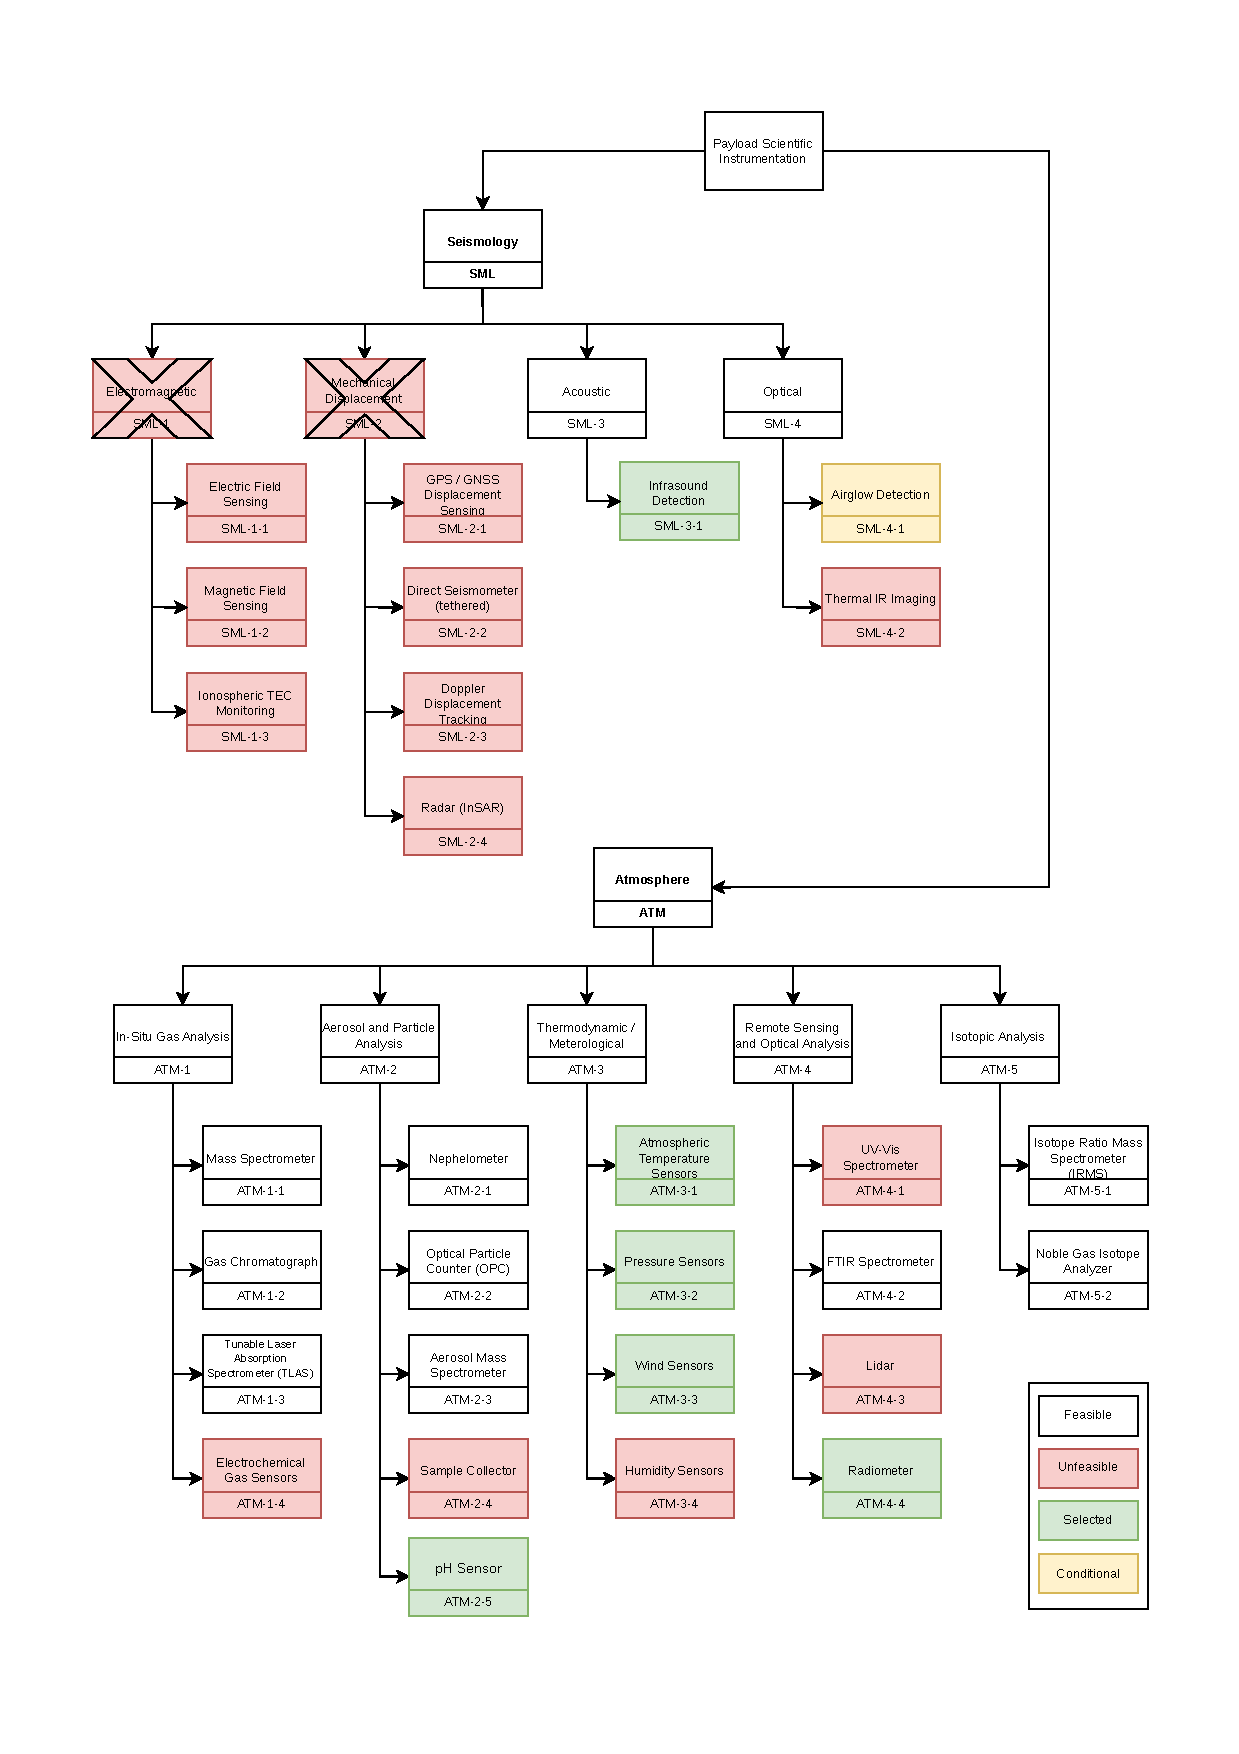
\includegraphics[
            page=1,
            width=\linewidth
        ]{fig/WFD-DOT_payload.drawio (2).pdf}
    \end{minipage}
    \vfill
    \begin{minipage}{\textwidth}
        \caption{Design Option Tree Payload Subsystem}
        \label{fig:dot_payload}
    \end{minipage}

\end{figure}


% \section{Instruments Trade-off}
% \label{sec:tradeoff_payload}
% Now that all instrument options have been presented, a trade-off to select the best techniques must be performed. The methods deemed infeasible in the previous section will not be considered in the trade-off. Due to the fact that some instruments are non-negotiable for satisfying the scientific requirements, they are automatically considered as part of the payload. Such instruments include: temperature sensors, pressure sensors, and wind sensors. The remaining 10 options fit different study categories and, although presented in the same table, are traded for different measurement purposes. There are four main groups of instruments that must be traded-off. The first refers to the atmospheric composition determination. Both a mass spectrometer and gas chromatography are able to accomplish the job, therefore a choice must be made. The second group refers to trace gas detection, where different techniques can be used to accomplish the similar results. The third ensures aerosol and particle characterisation, therefore a trade-off between nephelometer, an OPC and aerosol mass spectrometer must be performed. Finally, the fourth group refers to the isotopic analysis of the atmosphere. A choice must be made between using an IRMS or a noble gas isotope analyzer. 

% Different criterion for the trade-off have been established. That includes: scientific return of instrument, the corresponding TRL, mass, power consumption, reliability, and accuracy. Different weights are given to each criteria. The definition and scoring basis for each criterion is explained in \autoref{tab:tradeoff-criteria-payload}. The final atmospheric instruments trade-off table is presented in \autoref{trade-off-payload}. The different trade groups (1 through 4), as described above, are enumerated on the left side of the table for later reference. 

% % \begin{table}[H]
% % \centering
% % \caption{Trade-off criteria, definitions, and weights for balloon envelope material selection.}
% % \label{tab:tradeoff-criteria}
% % \footnotesize
% % \renewcommand{\arraystretch}{1.15}
% % \setlength{\tabcolsep}{4pt}
% % \begin{tabularx}{\linewidth}{@{}p{0.4cm} p{3.4cm} X p{1.0cm}@{}}
% % \toprule
% % \textbf{\#} & \textbf{Criterion} & \textbf{Definition and scoring basis} & \textbf{Weight} \\
% % \midrule
% % 1 & Scientific Return & Some instruments have higher scientific return than others and can provide multiple conclusions with fewer instrument combinations. This evaluates the amount of   & 30\% \\
% % 2 & TRL and flight heritage & TRL above 4 is a mission requirement, and the higher the TRL the better, therefore this is important criteria & 20 \% \\
% % 3 & Mass & Lower the mass the better, so important & 10\% \\
% % 4 & Power Consumption &  & 20\% \\
% % 5 & Reliability &  & 10\% \\
% % 6 & Accuracy &  & 10\% \\
% % \midrule
% % \multicolumn{3}{l}{\textit{Total}} & \textbf{100\%} \\
% % \bottomrule
% % \end{tabularx}
% % \end{table}


% \begin{table}[H]
% \centering
% \caption{Trade-off criteria, definitions, and weights for instrument selection.}
% \label{tab:tradeoff-criteria-payload}
% \footnotesize
% \renewcommand{\arraystretch}{1.15}
% \setlength{\tabcolsep}{4pt}
% \begin{tabularx}{\linewidth}{@{}p{0.4cm} p{3.4cm} X p{1.0cm}@{}}
% \toprule
% \textbf{\#} & \textbf{Criterion} & \textbf{Definition and scoring basis} & \textbf{Weight} \\
% \midrule

% 1 & Scientific Return &
% How directly and completely the instrument addresses the stated science objectives and VEXAG investigations, per REQ-STK-1.2. Score 1 (no direct link to any science objective) to 5 (crucial for VEXAG investigation and requirement compliance; removing it leaves a science objective entirely unaddressed).
% & 30\% \\
% \midrule

% 2 & TRL and Flight Heritage &
% Maturity of the instrument in Venus-relevant conditions. REQ-C-MIS-05 sets a hard minimum of TRL~4; instruments below this are non-compliant. Score 1 (TRL below 4) to 5 (TRL 8 and above, flight-demonstrated in Venus or directly analogous environment).
% & 20\% \\
% \midrule

% 3 & Mass &
% Instrument mass relative to the gondola cap of 200~kg (REQ-C-SUB-01). Score 1 (above 30~kg; incompatible with budget) to 5 (below 1~kg; negligible impact).
% & 10\% \\
% \midrule

% 4 & Power Consumption &
% Continuous power draw relative to the 500~Wh total energy storage cap shared across all subsystems (REQ-C-SUB-06). Weighted equally to TRL as it is the most crucial resource constraint. Score 1 (above 30~W; infeasible within budget) to 5 (below 1~W; negligible impact).
% & 20\% \\
% \midrule

% 5 & Reliability &
% Probability of sustained operation over the 5-year mission in the Venus H\textsubscript{2}SO\textsubscript{4} cloud environment, anchored to REQ-C-MIS-03 ($>$90\% survival) and REQ-C-PAY-01 ($>$80\% analysis success). Score 1 (likely to fail due to corrosion or mechanical wear within mission duration) to 5 (fully solid-state, no moving parts, no known H\textsubscript{2}SO\textsubscript{4} vulnerability).
% & 10\% \\
% \midrule

% 6 & Accuracy &
% Whether instrument precision meets the resolution required by the linked science objective under nominal Venus cloud deck operating conditions. Score 1 (precision insufficient to address the objective at any useful level) to 5 (precision exceeds the required resolution with comfortable margin under all expected conditions).
% & 10\% \\
% \midrule

% \multicolumn{3}{l}{\textit{Total}} & \textbf{100\%} \\
% \bottomrule
% \end{tabularx}
% \end{table}

% If any instruments present a scoring of 1 in any of the criterion, they are immediately discarded from the possible instrument options, as that means non compliance to the requirements. 

% \definecolor{score5}{RGB}{0,176,80}
% \definecolor{score4}{RGB}{146,208,80}
% \definecolor{score3}{RGB}{255,255,0}
% \definecolor{score2}{RGB}{255,192,0}
% \definecolor{score1}{RGB}{255,0,0}

% \begin{landscape}

% \scriptsize
% \renewcommand{\arraystretch}{1.35}
% \setlength{\tabcolsep}{2pt}

% \begin{longtable}{|
% >{\raggedright\arraybackslash}p{0.125cm}|
% >{\raggedright\arraybackslash}p{3.2cm}|
% >{\raggedright\arraybackslash}p{4.2cm}|
% >{\raggedright\arraybackslash}p{3.5cm}|
% >{\raggedright\arraybackslash}p{3cm}|
% >{\raggedright\arraybackslash}p{3.5cm}|
% >{\raggedright\arraybackslash}p{3cm}|
% >{\raggedright\arraybackslash}p{3.1cm}|
% >{\centering\arraybackslash}p{0.6cm}|}

% \caption{Instrument trade-off table}\\

% \hline
%  &
% \diagbox{\textbf{Instrument}}{\textbf{Criteria}}
% &
% \textbf{Scientific Return (30\%)}
% &
% \textbf{TRL (20\%)}
% &
% \textbf{Mass (10\%)}
% &
% \textbf{Power Consumption (20\%)}
% &
% \textbf{Reliability (10\%)}
% &
% \textbf{Accuracy (10\%)}
% &
% \textbf{Score}
% \\
% \hline
% \endfirsthead

% \hline
%  &
% \diagbox{\textbf{Instrument}}{\textbf{Criteria}}
% &
% \textbf{Scientific Return (30\%)}
% &
% \textbf{TRL (20\%)}
% &
% \textbf{Mass (10\%)}
% &
% \textbf{Power Consumption (20\%)}
% &
% \textbf{Reliability (10\%)}
% &
% \textbf{Accuracy (10\%)}
% &
% \textbf{Score}
% \\
% \hline
% \endhead

% % ---------------- MASS SPECTROMETER ----------------
% 1 &
% \textbf{Mass Spectrometer}
% & \cellcolor{score5!40}\textbf{5} Primary instrument for chemical composition and isotopic ratios
% & \cellcolor{score5!40}\textbf{5} Used previously in Venus and other space missions
% & \cellcolor{score2!40}\textbf{2} Among heavier instruments in the payload.
% & \cellcolor{score3!40}\textbf{3} Moderate power demand during active sampling.
% & \cellcolor{score5!40}\textbf{5} Flight-proven in Venus atmosphere.
% & \cellcolor{score5!40}\textbf{5} Very accurate chemical detection. 
% & \textbf{4.3}
% \\ \hline

% % ---------------- GC ----------------
% & 
% \textbf{Gas Chromatograph \cite{gas_chromo}}
% & \cellcolor{score3!40}\textbf{3} Limited identification capability.
% & \cellcolor{score5!40}\textbf{5} High TRL, tested previously in Venus missions.
% & \cellcolor{score2!40}\textbf{2} Among heavier instruments in the payload.
% & \cellcolor{score2!40}\textbf{2} High average power consumption.
% & \cellcolor{score4!40}\textbf{4} Heritage proven on previous missions.
% & \cellcolor{score4!40}\textbf{4} High resolution specs.
% & \textbf{3.0}
% \\ \hline


% % ---------------- IRMS ----------------
%  &
% \textbf{IRMS}
% & \cellcolor{score4!40}\textbf{4} Excellent for isotope analysis, but limited investigation scope.
% & \cellcolor{score3!40}\textbf{3} Venus-adapted IRMS not flight-demonstrated, development required.
% & \cellcolor{score2!40}\textbf{2} High mass.
% & \cellcolor{score3!40}\textbf{3} Moderate power, shares some hardware with mass spectrometer.
% & \cellcolor{score3!40}\textbf{3} Reduced reliability from history development gap.
% & \cellcolor{score5!40}\textbf{5} Extremely precise instrument.
% & \textbf{3.3}
% \\ \hline

% % ---------------- NOBLE GAS ----------------
% &
% \textbf{Noble Gas Isotope Analyzer}
% & \cellcolor{score3!40}\textbf{2} Limited identification capability.
% & \cellcolor{score3!40}\textbf{3} No Venus flight study, requires dedicated development.
% & \cellcolor{score2!40}\textbf{2} High mass, standalone instrument not shareable with mass spectrometer.
% & \cellcolor{score3!40}\textbf{3} Moderate power demand.
% & \cellcolor{score3!40}\textbf{3} Same development reliability concerns as IRMS.
% & \cellcolor{score2!40}\textbf{2} 
% & \textbf{2.8}
% \\ \hline

% \midrule

% % ---------------- TLAS ----------------
% 2 &
% \textbf{TLAS}
% & \cellcolor{score4!40}\textbf{4} High-sensitivity trace gas detection of SO\textsubscript{2}, HCl, H\textsubscript{2}O.
% & \cellcolor{score4!40}\textbf{4} High TRL but no Venus flight heritage.
% & \cellcolor{score4!40}\textbf{4} Compact solid-state design, lighter than other gas instruments.
% & \cellcolor{score4!40}\textbf{4} Low continuous power drawn.
% & \cellcolor{score4!40}\textbf{4} No moving parts, robust to vibration.
% & \cellcolor{score4!40}\textbf{4} Precision instrument for known gases 
% & \textbf{4}
% \\ \hline


% % ---------------- FTIR ----------------
% &
% \textbf{FTIR Spectrometer}
% & \cellcolor{score2!40}\textbf{2} Dense CO\textsubscript{2} saturates key IR bands.
% & \cellcolor{score4!40}\textbf{4} Mature technology but no Venus balloon study.
% & \cellcolor{score2!40}\textbf{2} Relatively heavy optical bench required.
% & \cellcolor{score3!40}\textbf{3} Moderate power, requires detector cooling.
% & \cellcolor{score3!40}\textbf{3} Interferometer moving mirror sensitive to vibration.
% & \cellcolor{score2!40}\textbf{2}Accurate but Venus conditions reduce effective retrieval quality.
% & \textbf{2.7}
% \\ \hline

% \midrule

% % ---------------- NEPHELOMETER ----------------
% 3 &
% \textbf{Nephelometer}
% & \cellcolor{score4!40}\textbf{4} Directly characterizes H\textsubscript{2}SO\textsubscript{4} cloud aerosol.
% & \cellcolor{score5!40}\textbf{5} Pioneer Venus heritage in identical environment.
% & \cellcolor{score4!40}\textbf{4} Lightweight optical instrument.
% & \cellcolor{score4!40}\textbf{4} Low power, passive scattering measurement.
% & \cellcolor{score5!40}\textbf{5} Extremely reliable, proven in Venus H\textsubscript{2}SO\textsubscript{4} clouds.
% & \cellcolor{score4!40}\textbf{4} Indirect inference of aerosol properties.
% & \textbf{4.3}
% \\ \hline

% % ---------------- OPC ----------------
% &
% \textbf{Optical Particle Counter (OPC)}
% & \cellcolor{score3!40}\textbf{3} Provides particle size distribution complementing nephelometer, not standalone.
% & \cellcolor{score4!40}\textbf{4} High TRL, however no Venus-specific testing.
% & \cellcolor{score5!40}\textbf{5} Very low mass.
% & \cellcolor{score5!40}\textbf{5} Negligible power consumption.
% & \cellcolor{score4!40}\textbf{4} Simple and robust optical design.
% & \cellcolor{score4!40}\textbf{4} 
% & \textbf{4.1}
% \\ \hline

% % ---------------- AEROSOL MS ----------------
% &
% \textbf{Aerosol Mass Spectrometer}
% & \cellcolor{score4!40}\textbf{4} Provides particle-level chemical composition beyond nephelometer capability.
% & \cellcolor{score3!40}\textbf{3} No Venus-specific heritage, adaptation required.
% & \cellcolor{score2!40}\textbf{2} Heaviest aerosol instrument option.
% & \cellcolor{score1!40}\textbf{1} High power demand limits compatibility with REQ-C-SUB-06.
% & \cellcolor{score2!40}\textbf{2} Reduced reliability from higher complexity and lack of testing in Venusian environment.
% & \cellcolor{score5!40}\textbf{5} Very accurate system.
% & \textbf{2.4}
% \\ \hline

% \midrule



% % % ---------------- RADIOMETER ----------------
% % \textbf{Radiometer}
% % & \cellcolor{score3!40}\textbf{3} Measures net IR radiative flux across cloud deck
% % & \cellcolor{score5!40}\textbf{5} Maximum maturity
% % & \cellcolor{score4!40}\textbf{4} Lightweight thermopile detectors.
% % & \cellcolor{score5!40}\textbf{5} Fully passive measurement, negligible power.
% % & \cellcolor{score5!40}\textbf{5} No moving parts, no environmental vulnerability.
% % & \cellcolor{score5!40}\textbf{5} Very simple, dual-unit nadir/zenith setup requires no active control.
% % & \textbf{4.4}
% % \\ \hline


% \end{longtable}

% \end{landscape}

\definecolor{score5}{RGB}{0,176,80}
\definecolor{score4}{RGB}{146,208,80}
\definecolor{score3}{RGB}{255,255,0}
\definecolor{score2}{RGB}{255,192,0}
\definecolor{score1}{RGB}{255,0,0}





\section{Instrument Selection}
\label{sec:instrument_selection}
% \autoref{tab:instruments} presents off the shelf models or estimate models from previous mission, in order to make a first estimation of the main budgets needed for the sizing of this as well as other subsystems. This includes the mass, power, and data rate budget, as well as, service temperature of each instrument, and corresponding volume. Nonetheless, most instruments will need modifications prior to the mission. 

% \begin{longtable}{%
%     p{3cm} |
%     p{2cm}
%     p{2cm}
%     p{2cm}
%     p{3cm}
%     p{2cm}
% }
% \caption{Payload Instrument Suite for a Venus 55~km Long-Duration Balloon Mission}
% \label{tab:venus_payload}\\
% \toprule
% \textbf{Instrument} &
% \textbf{Mass (kg)} &
% \textbf{Data Rate (kB/s)} &
% \textbf{Power (W)} &
% \textbf{Service Temperature\ ($^\circ$C)} &
% \textbf{Volume (cm$^3$)} \\
% \midrule
% \endfirsthead
% \toprule
% \textbf{Instrument} &
% \textbf{Mass (kg)} &
% \textbf{Data Rate (kB/s)} &
% \textbf{Power (W)} &
% \textbf{Service Temperature\ ($^\circ$C)} &
% \textbf{Volume (cm$^3$)} \\
% \midrule
% \endhead
% Neutral Mass Spectrometer (NMS) \cite{NMS} &
% 10.9 &
%  &
% 14 &
% $-20$ to $+50$ &
% 10650 \\
% \hline
% Auto-fluorescing Nephelometer (AFN) \cite{instruments} &
% 0.8 &
%  &
% 40 &
% $-10$ to $+40$ &
% 100 \\
% \hline
% % Particle Size Counter &
% % 0.45 &
% % 1 &
% % 1.5 &
% % $0$ to $+50$ &
% % --- \\
% \hline
% Weather Instrument Suite (WIS) \cite{instruments} &
% 0.1 &
% 0.05 &
% 1 &
% $-40$ to $+60$ &
% 98 \\
% \hline
% Sonic Anemometer \cite{Cheng2024StratosphericSonicAnemometer} &
% 3 &
%  &
% 5.3 &
% $-40$ to $+50$ &

% \\
% \hline
% Pressure Sensor (Barometer x5) \cite{barometers} & 0.450 & & 0.1 & -54 to +70 & 15.5
% \\
% \hline
% Mini Tunable Laser Spectrometer (mTLS) \cite{instruments} &
% 0.62 &
% 0.3  &
% 14 &
% $-40$ to $+80$ &
% 240 \\
% \hline
% Pyrgeometer \cite{pyro_radiometer} &
% 0.65 &
% 2.4 &
% 3 &
% $-40$ to $+80$ &
% 3530 \\
% \hline
% Tartu Observatory pH Sensor (TOPS) \cite{instruments} &
% 0.35 &
%  &
% 2 &
% $-20$ to $+50$ &
% 800 \\
% \bottomrule
% \end{longtable}

%bit rates are for telemtry, not necessarily raw data
%WIS data rate ranges from 7-400 bits/s depending on sampling. u can also do high sampling and then average with compression. This value is now for 1 every 10s 
%100 b/s to 3000 b/s based on sampling rate. for 2 Hz approximately 300 b/s
%mtls once every 4 hours
%tops 1 measurement every 10 seconds while it is on

%valus for NMS, AFN, mTLS, WIS, TOPS are sure
\begin{minipage}[t]{0.42\textwidth}
\small
\autoref{tab:instruments} presents off-the-shelf models or estimated models from previous missions in order to make a first estimation of the main budgets needed for the sizing of this and other subsystems. This includes the mass, power, data-rate budget, service temperature of each instrument, and corresponding volume. Nonetheless, most instruments will require modifications prior to the mission.
\end{minipage}
\hfill
\begin{minipage}[t]{0.54\textwidth}

\begin{table}[H]
\centering
\small
\setlength{\tabcolsep}{3pt}
\renewcommand{\arraystretch}{0.9}

\caption{Payload Instrument Suite for VISTA Mission}
\label{tab:venus_payload}

\begin{tabular}{lccccc}
\toprule
Instrument & 
Mass & 
Data & 
Power & 
Temp. & 
Vol. \\
& (kg) & (b/s) & (W) & ($^\circ$C) & (cm$^3$) \\
\midrule
NMS \cite{NMS} &
10.9 & 40\cite{hoffman1979pioneer} & 14 & -20 to 50 & 10650 \\
AFN \cite{instruments} &
0.8 & 1000\cite{baumgardner2022deducing} & 40 & -10 to 40 & 100 \\
WIS \cite{instruments} &
0.1 & 100 & 1 & -40 to 60 & 98 \\
Sonic Anemometer \cite{Cheng2024StratosphericSonicAnemometer} &
0.4 & 300 & 2 & -40 to 50 & 8000 \\
Barometers $\times5$ \cite{barometers} &
0.45 & 60 & 0.1 & -54 to 70 & 15.5 \\
mTLS \cite{instruments} &
0.62 & 500 & 14 & -40 to 80 & 240 \\
Pyrgeometer $\times2$ \cite{pyro_radiometer} &
0.65 & 300 & 3 & -40 to 80 & 3530 \\
TOPS \cite{instruments} &
0.35 & 800 & 2 & -20 to 50 & 800 \\
OPC \cite{OPC} & 
2 & 500 & 15 & -50 to 50 & 4500 \\
\bottomrule
\end{tabular}

\label{tab:instruments}
\end{table}

\end{minipage}
% ADD DUTY CYCLES, INTERVAL OF DATA GENERATION

\normalsize
\section{Sub-system Architectural Concepts}

Based on the instruments selected on the previous sections, different configuration arrangements can be considered for the gondola of the aerobot. Most instruments will be stored inside the gondola, where an inlet hole will connect them to the atmosphere when necessary. The pyrgeometers are required to be installed in a boom at a small distance from the gondola (around 10 cm). Moreover, the sonic anemometers also have part of its system sticking outside of the gondola, in order to determine the 3D vector of the wind. Therefore, the final 



\subsubsection*{Architecture A - Gondola Only}
All instruments are placed within the gondola, which is suspended beneath the balloon envelope. The gondola provides a controlled thermal and pressure environment, protecting sensitive electronics from the harsh Venusian atmosphere. Seismic detection will rely only in the barometers present within the gondola. While scientifically valid, this approach provides only indirect seismic sensing with limited localisation capability, and signal interpretation requires careful deconvolution from atmospheric noise. This architecture offers the highest instrument integration simplicity, lowest mechanical risk, and greatest thermal and pressure stability, making it the most robust baseline design.

\subsubsection*{Architecture B - Tethered Instruments}
Barometers are deployed along a tether hanging below the gondola, at varying lengths (15–300 m). By distributing pressure-sensing along the tether array, the system forms a vertical aperture that enables directional filtering of incoming acoustic-gravity wave signals. Cross-correlation of arrival-time differences between sensors at different altitudes allows triangulation of the wavefront bearing and, in combination with atmospheric propagation modelling, estimation of the seismic epicentre location. This significantly improves upon Architecture A's localisation capability. The tether design must account for Venusian wind shear at the cloud deck altitude, requiring careful dynamic analysis to avoid entanglement or resonance-driven oscillation. The tether and its sensor payload introduce additional mass and a deployment mechanism, raising complexity compared to Architecture A, but remain within heritage bounds of balloon tether systems tested in terrestrial stratospheric campaigns. This architecture represents a strong trade between enhanced science return and moderate additional mechanical risk. 

\subsubsection*{Architecture C - Towbody Probe}
A streamlined aeroshell probe, the towbody, is suspended on a long tether (1–60 km) below the balloon, descending beneath the Venusian cloud deck (\~48 km altitude) into the middle and lower atmosphere. The probe carries a dedicated instrument suite. Because the probe operates at higher pressures and temperatures than the balloon float altitude, it requires independent thermal protection and pressure vessel design, substantially increasing development complexity. The tether must sustain significant aerodynamic drag loads from differential winds between the float and probe altitudes, demanding careful materials selection and tether dynamics analysis. A separate power generating unit must also be considered. This architecture offers the most scientifically ambitious capability, with direct in-situ sub-cloud measurements as well as more seismic sensitivity due to closer proximity to the surface. However, it carries the highest mass, mechanical, and thermal risk of the three architectures, and the long tether introduces potential balloon stability perturbations that must be assessed through coupled flight dynamics modeling. 

\section{Subsystem architecture Trade-Off}
\label{sec:payload_tradeoff}
Given the three architectures presented in the previous section, a trade-off must now be performed in order to choose the selected instrument's payload final architecture. Five criteria were chosen with a corresponding attributed weight. The criteria with highest weight are related to their scientific value to the mission: Science Return (25\%) and Seismic Localisation (30\%). The remaining criteria are: Mission Risk (15\%), Mass \& Complexity (15\%), and Heritage \& Feasibility (15\%). They all carry equal weight, as they have shared importance as mission-enabling constraints. Finally, a score system is used in order to compute the best architecture. The scoring works as follows: \textbf{1} = severe deficiency, unfeasible; \textbf{2} = partial deficiency; \textbf{3} = meets requirement; \textbf{4} = exceeds requirement; \textbf{5} = significantly exceeds requirement. If any architecture presents score 1 in any criteria, they will be immediately discarded, despite the remaining scores in the other criteria. 



% Softer pastel palette
\definecolor{score1}{RGB}{242,180,180}   % pastel red
\definecolor{score2}{RGB}{245,205,160}   % pastel orange
\definecolor{score3}{RGB}{250,235,170}   % pastel yellow
\definecolor{score4}{RGB}{210,235,200}   % pastel green
\definecolor{score5}{RGB}{170,220,170}   % stronger pastel green

% All text black
\newcommand{\sone}[1]{\cellcolor{score1}\color{black}#1}
\newcommand{\stwo}[1]{\cellcolor{score2}\color{black}#1}
\newcommand{\sthree}[1]{\cellcolor{score3}\color{black}#1}
\newcommand{\sfour}[1]{\cellcolor{score4}\color{black}#1}
\newcommand{\sfive}[1]{\cellcolor{score5}\color{black}#1}

\begin{table}[htbp]
\centering
\caption{Instrument subsystem architecture trade-off}
\label{tab:arch_tradeoff}

% Smaller + tighter
\scriptsize
\renewcommand{\arraystretch}{1.15}
\setlength{\tabcolsep}{3pt}

\begin{tabular}{
  p{1.3cm}
  p{2.8cm}
  p{2.4cm}
  p{3.0cm}
  p{2.3cm}
  p{2.3cm}
  p{0.8cm}
}
\toprule
\textbf{Arch.}
  & \makecell[l]{\textbf{Science}\\\textbf{Return}\\\textbf{(25\%)}}
  & \makecell[l]{\textbf{Mission}\\\textbf{Risk}\\\textbf{(15\%)}}
  & \makecell[l]{\textbf{Seismic}\\\textbf{Localisation}\\\textbf{(30\%)}}
  & \makecell[l]{\textbf{Mass \&}\\\textbf{Complexity}\\\textbf{(15\%)}}
  & \makecell[l]{\textbf{Heritage \&}\\\textbf{Feasibility}\\\textbf{(15\%)}}
  & \makecell[l]{\textbf{Score}} \\
\midrule

\textbf{A} Gondola Only
  & \sthree{\textbf{3} Meets all atmospheric REQs; no spatial dynamics measurement.}
  & \sfive{\textbf{5} No deployables; lowest mechanical failure risk.}
  & \stwo{\textbf{2} Internal barometers only; epicentre localisation not achievable.}
  & \sfive{\textbf{5} Minimum mass; no deployment mechanism.}
  & \sfour{\textbf{4} Vega heritage; with TRL\,$\geq$\,5.}
  & \textbf{3.45} \\

\midrule

\textbf{B} Tethered Instruments
  & \sfour{\textbf{4} Meets all atmospheric REQs; tether array adds vertical wind-shear and cloud dynamics data.}
  & \sthree{\textbf{3} Tether oscillation risk mitigated by heritage, additional failure mode during deployment.}
  & \sfour{\textbf{4} Vertical baseline enables wavefront triangulation; estimation of epicentre localisation achieved.}
  & \sfour{\textbf{4} Moderate mass and deployment complexity; within budget.}
  & \sthree{\textbf{3} Stratospheric tether heritage; Venus-specific qualification needed.}
  & \textbf{3.7} \\

\midrule

\textbf{C} Towbody Probe
  & \sfive{\textbf{5} Sub-cloud in-situ chemistry and dynamics.}
  & \sone{\textbf{1} Multiple failure modes, with tether, thermal, and power risks being mission-critical.}
  & \sfive{\textbf{5} Surface proximity maximises infrasound amplitude and localisation accuracy.}
  & \sone{\textbf{1} Highest mass and complexity, likely violates mass budget.}
  & \stwo{\textbf{2} No Venus heritage for long-tether towbody; with TRL\,$\leq$\,3.}
  & \textbf{3.35} \\

\bottomrule
\end{tabular}
\end{table}

After performing the subsystem configuration trade-off, architecture B is the winning one. This is mainly due to its high scientific value at a low mass and complexity cost. Architecture A is a strong contender, however not the selected one. Architecture C, on the other hand, is eliminated due to its score of 1 in two criteria, making it unfeasible for the VISTA mission. 

\section{Final Payload subsystem architecture description}



\begin{figure}[H]
\centering

\begin{minipage}[t]{0.67\textwidth}
\vspace{0pt}

In architecture B deploys three barometers along a tether suspended beneath the gondola, at separations of 15,m, 85,m, and 200,m. The gondola stores the primary atmospheric instruments alongside two additional barometers and an IMU (also shared with other subsystems), the latter providing attitude and acceleration data to decouple gondola motion from atmospheric pressure fluctuations. Power and communications lines to each node are accommodated within the tether cable, whose material selection is addressed in the structures subsystem. The tether deployment mechanism is outside the current design scope and will be treated in subsequent stages.
The three tethered barometers, in addition to providing a vertical aperture array for seismic localisation, offer redundancy against individual node failure. Cross-correlation of infrasound arrival-time differences across the five-barometer baseline (three tethered, two in the gondola) enables triangulation of acoustic-gravity wavefronts and rough estimation of seismic epicentre location. The precise in-flight altitude of each node depends on tether dynamics under Venusian wind shear and is subject of subsequent design stages.

\end{minipage}
\hfill
\begin{minipage}[t]{0.28\textwidth}
\vspace{0pt}
\centering
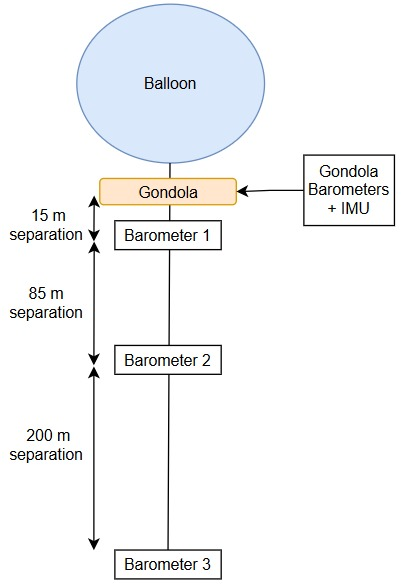
\includegraphics[width=\linewidth]{fig/archB_payload.png}
\caption{Architecture B}
\label{fig:placeholder}
\end{minipage}

\end{figure}

\section{Verification and Validation}

\section{Sensitivity Analysis}
